\chapter{Deus et Eliseus Ascenderunt in Caelum}
\begin{center}
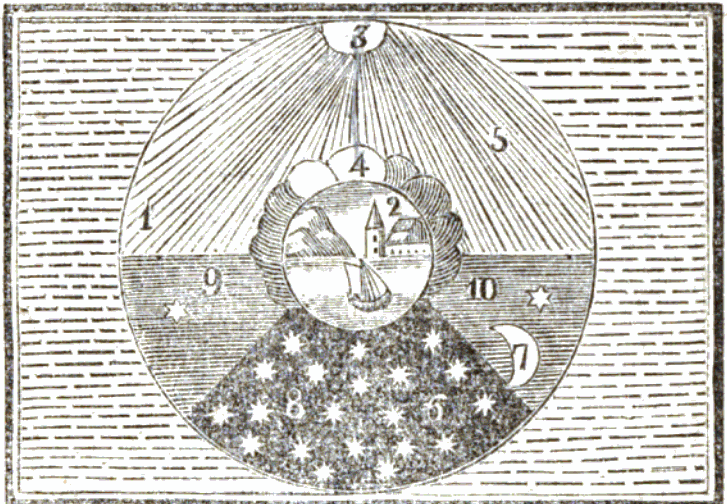
\includegraphics[scale=1.5]{Heaven.png}
\end{center}

\section{Intended Audience}
This is intended for students who have completed Lectio 5 and 6 of Latin by the Natural Method and Chapter 5 of Lingua Latina Per Se Illustrata. There are words in this chapter.

\section{Text}
Deinde Deus misit Eliseum in Caelum, misit eum in terra. Deus deinde relinquit Eliseum Solum in terra. Eliseus solus non scivit locum in quo fuit. Deinde, Eliseus vidit virum. Eliseus ambulavit ad virum. Vir fuit propheta Jeremias. "Salve" Eliseus dixit ad eum "Quomodo te habes?". "Bene valeo" dixit Jeremias, "Ut valesne?" interrogavit. "Male valeo" dixit Eliseus. "Cur?" Jeremias interrogavit. "Quia" inquit Eliseus "Non video Deum, sicut Vidi eum". "Quare tristus es? Num scis Deum in locis omnibus esse?". "Ita" respondit "Sed si non video eum, quomodo laetificor?". "Sede, facio ignem." \par 

Jeremias accepit Chalybem. Cum chalybe in manu sua, pulsavit silicem cum chalybe. Deinde ex silice scintilla volavit in suscitabulum. In suscitabulo, fumus ascendit in caelum. Deinde, Jeremias posuit silicem et chalybem in terra. Eliseus aspexit silicem et chalybem. Chalybs est durus est et etiam silex. Eliseus vidit silicem quando pater eius fecit ignem. 

\footnote{\textbf{Laudēs} = Lauds (Morning Prayer)}

